\documentclass[a4paper,UTF8]{ctexart}
\usepackage{graphicx}
\usepackage[a4paper,top=3cm,bottom=2cm,left=3cm,right=3cm,marginparwidth=1.75cm]{geometry}
\CTEXsetup[format={\Large\bfseries}]{section}
\title { \bfseries \huge 网络编程实验报告}
\author{
		 实验名称:~\makebox[10em][c]{网络编程第一次作业}\\
		 实验日期:\makebox[10em][c]{2020/5/1}\\
	 	 学生姓名:\makebox[10em][c]{杨彬}\\
	 	 学生学号:\makebox[10em][c]{09017423}\\
		}
\date{}

\begin{document}

\maketitle

	\section[aligh=left]{实验目的}
		\begin{enumerate}
			\item 实验 1-1 :使用Freebsd/Linux操作系统下的C编译器和网络程序的调试方法,掌握TCP连接建立和终止以及调整缓冲区大小的方法
			\item 实验 1-2: 使用ethereal/TCPDump等抓包工具,截取TCP建立过程中产生的数据包,分析连接建立过程。
		\end{enumerate}
	\section {实验环境}
		\par ubuntu 18.04 , gcc 7.5.0
	\section {实验内容}
		\subsection{实验1-1}
			\subsubsection{实验思路}
				\begin{enumerate}
					\item 修改 datetimec.c 和 datetimes.c 的源代码。因为源代码原本使用的是13端口,修改源代码将端口换为12000端口
					\item 编译 datetimec.c 为client 和 datetimems,c 为 server
					\item 先运行 server 再运行 client
				\end{enumerate}
		\subsection{实验1-2}
					\subsubsection{实验思路}
				\begin{enumerate}
					\item 使用命令 \verb|sudo tcpdump -i lo port 12000 -vvv -w ./segment| 监听本地通信,并将抓到的包保存到指定目录下
					\item 在 实验 1.1 的基础上,先运行 server 在运行 client
					\item 用 wireshark 或者 tcpdump 分析抓到的包分析连接的建立过程
				\end{enumerate}
	\section {实验结果分析及讨论}
		\subsection{实验1-1}
		\subsubsection{datetime程序运行}
			运行编译得到的 client 和 server 得到如下结果
			\begin{figure}[h]
				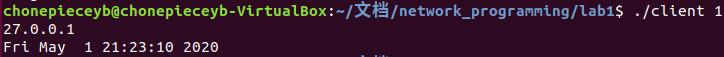
\includegraphics[scale =0.7]{./resources/1.jpg}
				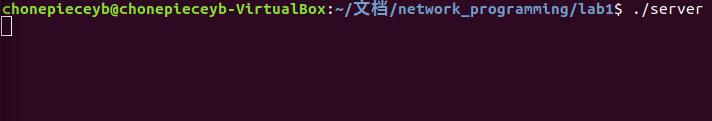
\includegraphics[scale =0.7]{./resources/2.jpg}
				\caption{实验1-1结果}
				\end{figure}

		\subsubsection{TCP状态图分析}
		\begin{figure}[htb]
			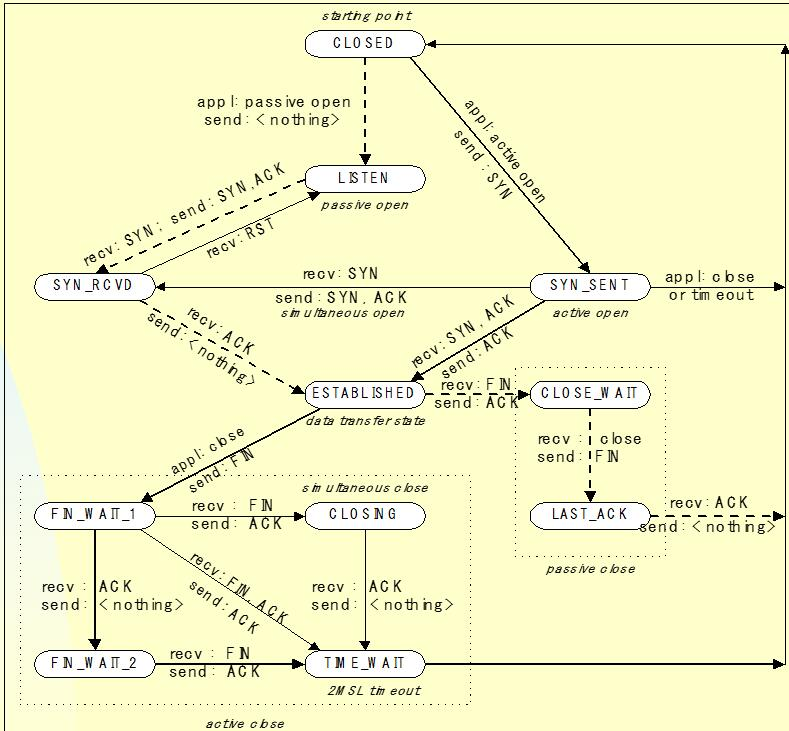
\includegraphics [scale=0.6]{./resources/3.jpg}
			\caption{tcp连接状态图}
		\end{figure}
		\par 对TCP连接状态图做简要总结,对于正常的 tcp连接一般由客户端发起连接请求(也称为 active open),服务端监听请求(passive open)。在关闭连接的时候,由客户端或者服务端某一方先发送 fin 包 请求关闭连接(先发送 fin 包的一方的连接是 active close 一般是客户端),相对的另外一方接收 fin 包的为 passive close。其建立连接和关闭连接的过程如下;
		\par 建立连接,三次握手
		\begin{enumerate}
			\item 第一次握手,client 发送 syn 包,发起连接请求,设置 client 的 ISN (initial sequence number),由 $CLOSED$ 状态转入 $SYN_SENT$状态; 
			\item 第二次握手,server 直接由 CLOSED状态进入 LISTEN状态,监听连接请求,一旦收到client 发送的 syn包,server端 发送 [syn,ack] 包 ,设置 server 的 ISN 同时 回应(ack) client 发送的 syn 包, server 由 $LISTENED$ 状态进入到 $SYN_RCVD$状态
			\item 第三次握手,client 收到 server 发送的 [syn,ack] 包, 发送 ack 包回应server, client 由 $SYN_SENT$状态进入$ESTABLISHED$状态,server在收到 client 的 ack 包之后 由 $SYN_RCVD$状态进入$ESTABLISHED$状态,三次握手完成,server client都互相知晓对方的LSN,连接建立完成
		\end{enumerate}
		\par 关闭连接,四次挥手,假设由 client 先发送 fin
		\begin{enumerate}
		\item 第一次挥手 client 发送 [fin] 包,表明 client 的数据已经全部传送完毕,client 由 $ESTABLISH$状态进入$FIN_WAIT1$状态。
		\item 第二次挥手 server 收到 client 发送的 fin 包后,知道 client 的数据已经发生完毕,向客户端发送 ack 包,从 $ESTABLISH$ 状态进入到 $CLOSE_WAIT$状态,等待server自身数据发送完成, client 收到 ack之后 由 $FIN_WAIT1$状态变为$FIN_WAIT2$状态。在server发送 $FIN$之前,client仍然可以接收server发送的数据,但client不能再发送数据,这种状态就成为TCP的半连接状态
		\item 第三次挥手 server确认自己已经发送完所有的数据之后,发送 fin 包给服务端,告知client自己没有数据要发送了。server 由 $CLOSSE_WAIT$状态变为$LAST_ACK$状态。等待client的ack,最终关闭。
		\item 第四次挥手 client收到 server 的 fin包之后,发送 ack,进入 $TIME_WAIT$状态,在等待两个 MLT 之后进入 $CLOSE$状态。而 server在收到 ack 之后进入 $CLOSE$状态,设置 $TIME_WAIT$状态的目的是 1 当最后一个 ack 丢包,client能然可以重传ack 2. 防止当前的socket被复用(在连接关闭之后,马上建立四元组相同的新的连接),导致出错。
		\end{enumerate}
	\subsubsection{实验1-2}
		\subsubsection{用tcpdump抓包结果}
			\begin{figure}[htb]
			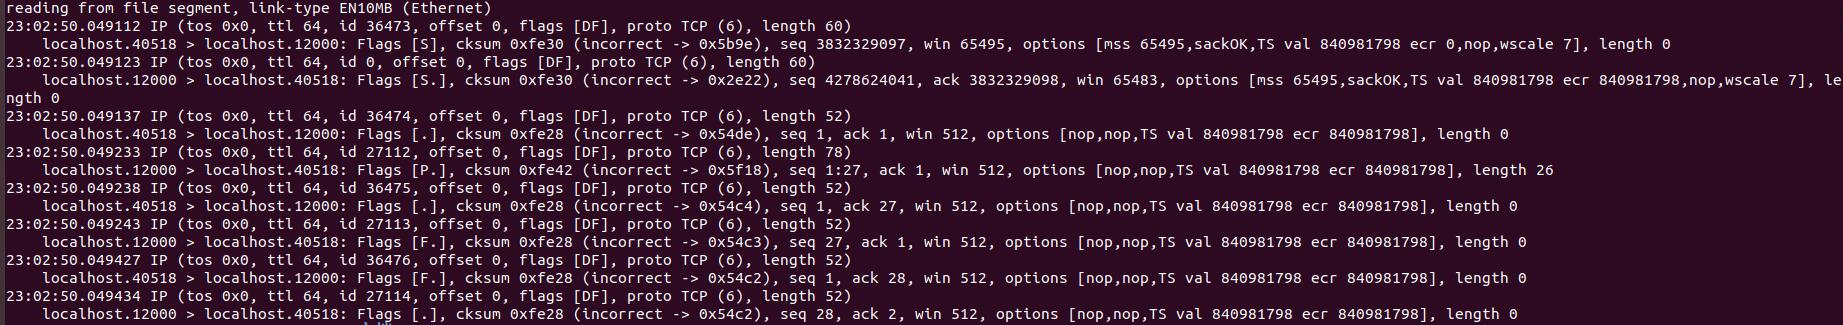
\includegraphics[scale=0.4]{./resources/4.jpg}
			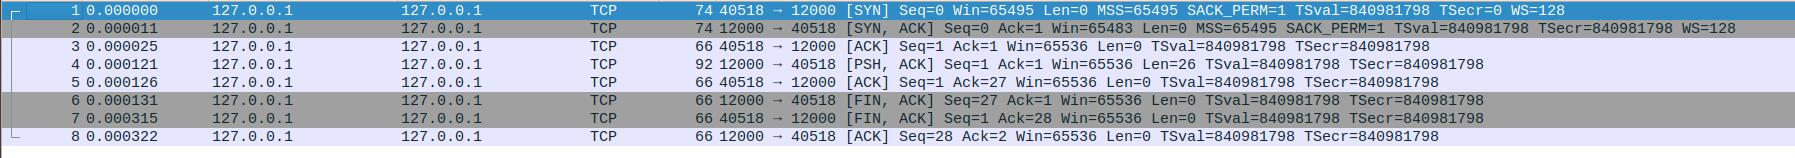
\includegraphics[scale =0.4]{./resources/5.jpg}
			\caption{tcp抓包结果}
			\end{figure}
		\subsubsection{抓包分析}
		\par 三次握手包
		\begin{enumerate}
			\item 1 号包, 第一次握手由 client 发送给 server ,seq为799005335,表示 ISN为该值,flag 中有 syn标志,表明这是一个同步包
			\item 2 号包, 第二次握手由 server 发送给 client , seq为2266925295。表示server方的ISN为该值,flag中有 syn和 ack 标记, ack的值为 client的LSN+1(syn占一个序号)。第二次握手包同时发送了 syn和ack
			\item 3 号包,第三次握手,由client 发送给server,对 server发送的 syn包进行回应,该包syn的大小为 server的 ISN+1。
		\end{enumerate}
		\par 四次挥手包
		\begin{enumerate}
			\item 6 号包,第一次挥手包,有 client  发送 fin 包给 server
			\item 7 号包,第二次和第三次挥手,由于 server端发送完数据之后,直接关闭,因此直接将第二次和第三次挥手合并。发送 [ack,fin] 包给client,回应 client 的 fin包,同时发送 server的fin包
			\item 8 号包, 第四次挥手,client收到 server发送的 fin包之后,发送 ack回复。进入time wait 状态,server收到 ack之后连接关闭。
		\end{enumerate}
\end{document}